\documentclass[10pt, onecolumn]{article}

\usepackage[utf8]{inputenc}
%\renewcommand*{\familydefault}{\sfdefault}

\usepackage{amsmath, amssymb}

\usepackage{graphicx}
\usepackage{fullpage}
\usepackage{algpseudocode}

\newcommand{\U}{\mathcal{U}}
\renewcommand{\L}{\mathcal{L}}
\newcommand{\newx}{{x}}
\newcommand{\newy}{y}
\newcommand{\answer}{h}
\renewcommand{\H}{\mathcal{H}}
\newcommand{\R}{\mathbb{R}}
\newcommand{\X}{\mathcal{X}}
\newcommand{\D}{\mathcal{D}}
\newcommand{\C}{\mathcal{Y}}


\usepackage{lineno}

%\linenumbers

\usepackage[numbers, square, sort]{natbib}

\usepackage{framed}

\parindent0pt
\parskip5pt


\begin{document}
% % % % % % % % % % % % % % % % % % % % % % % % % % % % % % % % % % % % % % % %
%\title{A model for the labeller in active learning: Accounting for "I
%  don't know" and "not this"}
\title{Labeller adjusted active learning: Accounting for "I
  don't know?!?" and "Definitely not this!"}
\author{A1, A2}
\maketitle


\begin{abstract}
We discuss the active learning of a classifier when 1) a labeller
returns a probability vector over the labels 2) the labeller's
certainty of the labels is not constant over the item space. We show
how the labeller uncertainty can be modelled using Gaussian process
latent variable model, and how incorporating the uncertain labeller
model to the optimal sampling scheme improves classification under
uncertain labeling.
\end{abstract}


\section{Introduction}

The optimal design of sampling for improving model estimates, also
known as active learning, is a popular method for training classifiers
on large collection of items. In short, an unlabelled item database is
ranked based on the usefullness of the expected label for the current
state of the classifier. Then an external human labeller is asked for
the correct label and the model is re-estimated. In theory, the
learning rate of the classifier is optimal as the data so collected is
the most useful. 

The process relies on the labeller ability to produce the correct
label, hence the often used name 'oracle'. The oracle is assumed
all-knowing, and several approaches have been introduced to alleviate
this unrealistic assumption. In general, the label is allowed to be
wrong with some probability, reflecting e.g. the limited knowledge of
the labeller.

The five papers studying labellers with imperfect answers [][][]][]
assume the following: ... 


In this paper we discuss two novel ideas. First, we want to
accommodate the answers "definitely not this one" and "I don't
know". Second, we want to account for the user's limited knowledge in
the active learning process. 



% \section{Related work}

% ``Realistic-ness of assumptions for the labeller'' (in increasing
% order):
% \begin{description}
%   \item [oracle:] knows everything; returns one true class label
%   \item [noisey oracle:] knows everything, but with an error; returns
%     one class label, with an error
%   \item [our model:] 
% \end{description}

% (Recap: oracle, noisy oracle, Yan++.)



\section{Outline of approach}
\label{sec:outline}

As the core problem of interest we tackle the training of a classifier
in a semi-supervised manner. We have a set of labeled training items,
and we want to improve the classifier by querying an external labeller
for some more labels for unlabeled items. The idea is that asking is
expensive, so we should only query the most useful items \textit{given
the classifier and the labeller} at hand.

Formally, let $\D=\{i=(y_i,x_i)\}$ denote a set of items, where
$y_i\in \C$ with $|\C|=K$ denote labels for the items and $x_i\in
\X\subseteq \R^p$ denote other features. Write for any $x\in\D\cap \X$
the correct label $y_x$. We assume the pool-based sampling scheme,
i.e. we have a pool $\U\subset D\cap \X$ of unlabeled items which we
can use for querying the labeller for their labels. We assume that the
cost of querying is constant. 

Our proposed approach, coined \textit{labeller adjusted uncertainty
  sampling}, can be outlined by the following schematic algorithm
\citep[cf. ``prototypical active learning algorithm''
presented by][]{Olsson@2009}:
\begin{algorithmic}[1]
  \State Initialize $\L = \L_0 \subset D$
  \While{Some stopping criterion is not met}
    \State Train classifier $c$ with a set of correcly labeled items $\L$
    \State Select unlabeled item $x^* \in \U$ based on the highest
      \textit{labeller adjusted informativeness}:
      \State \qquad Estimate informativeness of $x \in \U$ for the
        classifier $c$ 
      \State \qquad Estimate uncertainty of $x \in \U$ for the
        labeller $l$
      \State \qquad Combine both measures  
    \State Query labeller for the label $y^*_{x^*}$ of $x^*$; add
      $(y^*_{x^*}, x^*)$ to $\L$ 
  \EndWhile
  \State Return final classifier $c$
\end{algorithmic}

This is an extension of the well-known ``uncertainty sampling
strategy''. However, instead of only taking the classifier's into
account, we also take the knowledge of the labeller into account.

This introduces three challenges which we address in detail in the
subsequent sections. First, we need a way to enable the labeller to
give flexible answers, e.g., to return ``I don't know'' or ``I am sure
it is this label'' (line~8 in the algorithm, discussed in
Section~\ref{sec:answers}). Second, we need a model to estimate the
labeller's uncertainty for a possible candidate query (line~6,
Section~\ref{sec:labeller}). And, third, we need a suitable way to
combine the classifier's informativeness and the labeller's
uncertainty (line~7, Section~\ref{sec:adjustment}).


\paragraph{Example.} Throughout the paper we use a simple
two-dimensional example to illustrate each challenge and our proposed
solution. For the item set $D$ we simulated three 2D Gaussian
clusters, 50 points each; Figure~\ref{fig:sampling1}(left) shows the
data set with the ground-truth labels. We use the Naive Bayes
classifier with Gaussian distributions as the base classifier.



\section{A model for flexible answers}
\label{sec:answers}

We assume that a classifier is used that can be written as
\begin{eqnarray}
y | x, \theta &\sim & p(y| x, \theta)=\prod_k p(k|x,\theta)^{[y=k]}\\
\theta & \sim & p(\theta)
\end{eqnarray}
with $\theta$ being the parameters of the model, and $p(\theta)$
denoting a prior distribution for the parameters. We define that for
each query, the labeller returns a probability vector $\answer_x \in
\H=\{h\in \R_+: \sum_{k\in \C} h_k=1\}$. We furthermore assume that
the labeller is biased towards the correct label,
i.e. $\mathrm{argmax}_k h_{xk}=y_x$.

The oracle labeller is then the special case ''definitely $k$'' with
$h=\mathbf{1}\{h_k=1\}$. The "I don't know" case is $\mathbf{1}\{
h_k=K^{-1}\ \forall k\}$, and in between are a continuum of
alternatives, including the "definitely not $k$" with
$\mathbf{1}\{h_k=0\}$ and "one of these $M$" with $\mathbf{1}\{h_k>0\
\forall k\in M\}$. 

The connection between $h$ and $y$ needs to be made in order for the
extension to be useful in learning the classifier parameters
$\theta$. We assume that the following model is valid: 
\begin{eqnarray}
\label{eq:ph}
p(h|x, \theta)&\propto&p(h|x) \prod_k p(k|x, \theta)^{h_k}
\end{eqnarray}
in which the $y$ variable is no longer necessary to be observed. The
model is a continuous version of  categorical model, and as $y$ is a
categorical variable, we can replace the observations $y$ with
indicator vector $\mathbf{1}(h_y=1)$. An interpretation for the
approach is given by the multinomial distribution: the product is
approximately the likelihood of a multinomial variable if $h$ would be
integers. The scaling of $h$ is not important, the pairwise
proportions of $h_k$ are the main information. As a practical example,
the user could be given a set of ten tokens to distribute among the
label candidates.


\paragraph{Example.} To illustrate this approach, we
conducted a simulation study with our two-dimensional toy data
set. The parameters $\theta=\{\mu_k, \Sigma_k: k=1,...,K\}$ for the
Naive Bayes classifier for a given set of observations
$L=\{(h_i;x_i)\}$ are given as weighted averages and covariance
matrices, i.e. each queried item $x_i$ is 'observed' in each of the
$K$ classes with a weight $h_i$. Two points from each cluster were
given as the initial data for the classifier.

We simulated two labeller. Both knew one of the classes, say $k'$, and
when queried with an item of this class they returned a corresponding
indicator vector. When queried with an item of another classes one
labeller returned $0.5$ for $k\neq k'$ (and 0 for $k'$ as the labeller
knows the label is not $k'$). The other labeller was forced to make a
decision, simulated here by a random pick.
 
We ran 20 different samplings sequences from the item set, each step
drawing uniformly from the pool of unlabeled items. The classification
rate over a test set for the forced-to-choose labeller were averaged
over 10 random picking sequences per sampling, estimating the
expectation over the forcing event. Figure \ref{fig:sampling1}(right)
shows the $(0.05, 0.5, 0.95)$ quantile envelope plots of the
classification rate as a function of sample size.
  
\begin{figure}[hbtp]
\centering
\includegraphics[width=3in]{figures/data.pdf}
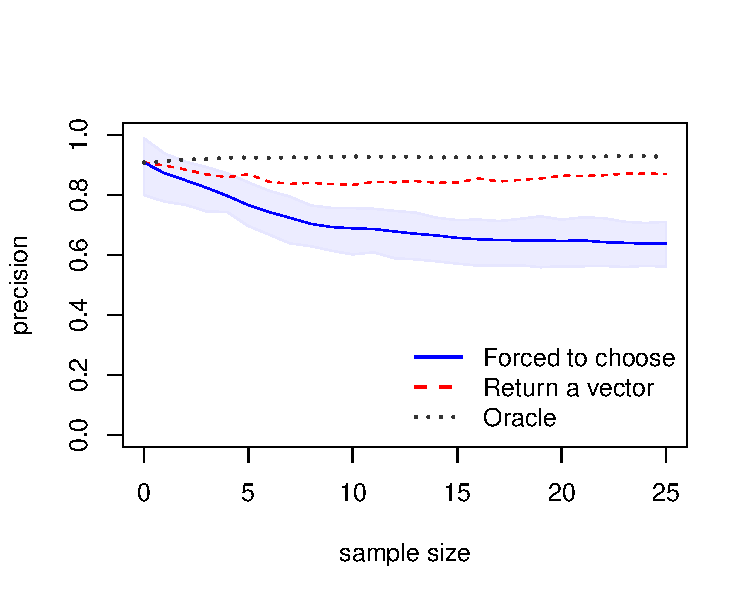
\includegraphics[width=3in]{figures/choose1_vs_give_vector.pdf}
\caption{Classification rate example, two modes the user can provide
  labeling information: Choose one vs. a weight vector. The shaded
  area is the 90\% range over data sampling sequences, 20 different
  samplings. The forced-to-choose values are further averaged over 10
  random selection sequences per sampling sequence.}
 \label{fig:sampling1}
\end{figure}

The illustration nicely shows that the is improved if the labeller is
allowed to express uncertainty for a query and is not forced to choose
a single value. This allows us to model the labeller's uncertainty.



\section{The answer depends on the question}
\label{sec:labeller}

Obviously, the uncertainty of a labeller depends on the specific query
which item $x$ to label. Therefore, we assume that $\alpha(x)\in \R$
is a value that describes the uncertainty the labeller has on the
label of $x$, and assume that $\alpha$ is continuous and varies
smoothly in $\X$. The interpretation is that high value of $\alpha$
means high uncertainty, and vice versa.  

Continuing from the Equation~\ref{eq:ph}, we now introduce a prior for
the $h$ values. We model them as dependent on the smooth $\alpha$,
which we assume in this paper to be adequately described by a
log-Gaussian process in $\X$. The natural model for $h$ is the
Dirichlet distribution, we simplify the problem by assuming symmetry,
i.e., the Dirichlet parameter $\alpha$ is the same for all classes. 

The prior $p(h|x,\alpha)$ for the labeller's variable output then
becomes 
\begin{eqnarray}
h | x, \alpha &\sim& Dir(\alpha(x))\\
\alpha &\sim & \log{-GP(\mu, C)}
\end{eqnarray}
with some hyper-prior mean $\mu$ and covariance function $C$. In what
follows the parameter $\alpha$ shall be known as the \emph{labeller's
  uncertainty}. 


\paragraph{Example.} We simulated a labeller with a circular "area of
expertice", a disc in the feature space within which the labeller
knows the labels. Outside the labeller returns "I don't
know". Figure~\ref{fig:est_alpha1} depicts the Kriging surface
estimate of $\alpha$ after 10 and 20 uniformly chosen queries. 

\begin{figure}[hbtp]
\centering
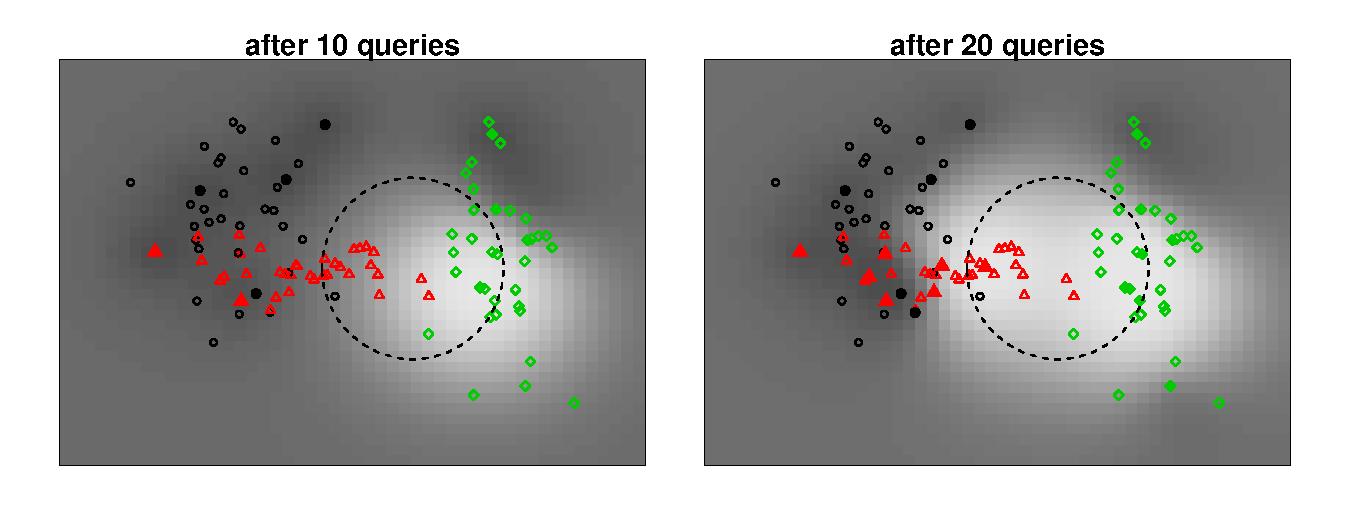
\includegraphics[width=6in]{figures/estimated_alpha.pdf}
\caption{Labeller's uncertainty as estimated after 10 (left) and 20
  (right) queries. Symbols denote the item set, filled symbols
  indicate items that were queried. The Dashed disc is the labeller's
  area of expertice where he knows the label. Dark color of the
  background is for low certainty areas and light color is for high
  certainty areas of the feature space.}
\label{fig:est_alpha1}
\end{figure}

Being now able to detect the area of expertice of a labeller, an
immediate question arises: How can we combine the two models in order
to do active learning? 

% For optimal result the classifier itself would account for the
% labeller's uncertainty, but unfortunately the hierarchical nature of
% the labeller model is not trivial to implement. For simplicity of
% implementation we will focus our discussion on the case where the
% labeller model is independent from the classifier model.



\section{Informativeness estimation and adjustment}
\label{sec:adjustment}

Here, we focus our discussion on the case where the labeller model is
independent from the classifier model, i.e., not the classifier itself
takes the labeller's uncertainty into accout, but we combine the
classifier's informativness and the labeller's uncertainty in a
reasonable way.

As outlined in Section~\ref{sec:outline}, in every iteration of the
algorithm the model parameter estimates are used for computing an
informativeness function $I(x)=I(x;\hat\theta)$ (line~5). This
provides a measure of usefulness of gaining the label of an item $x\in
\U$. There exists several formulations of $I(x)$, we will focus on the
entropy,
\begin{eqnarray}
I_c(x)&:=&-E_y [\log p(y|x,\hat\theta)]\\ 
&=&-\sum_k p(k|x,\hat\theta)\log p(k|x,\hat\theta)
\end{eqnarray}
where the probabilities are the posterior predictive probabilities at
the current iteration. Note, that the uncertainty sampling strategy
then queries the item which maximizes this informativeness $I_c$.

Because of the knowledge (or better not-knowledge) of the labeller who
maybe does not always know the label, the expected gains are reduced.
The informativeness given by the labeller can also be expressed using
the entropy,
\begin{eqnarray}
I_l(x)&:=& -E_h \log p(h|x, \L)
\end{eqnarray}
where $\L$ is all so far collected data. The entropy of a Dirichlet
distributed $h$ depends on the $\alpha$, leading to the formula
\begin{eqnarray}
I_e(x)&=& E\left\{ \log B(\alpha(x)) + \right. \\
& &\left. K(\alpha(x)-1)[\psi(K\alpha(x))-\psi(\alpha(x))] \right\}\nonumber
\end{eqnarray}
where $B$ is the beta-function, $\psi$ is the digamma function, and
the expectation is over $\alpha(x)$. Unfortunately this function is
not monotonous in $\alpha$, as the $h$ will converge to uniform as
$\alpha$ increases, and the entropy decreases. Uniform $h$ should be
regarded as the least informative answer from the labeller. We
therefore suggest the use of variance which is a monotonically
decreasing function of $\alpha$,
\[
I_l(x):= Var [h|x, \alpha] = \frac{K-1}{K^2(K\alpha(x)+1)}.
\] 

The two $I(\cdot)_{\cdot}$ functions do not share units, to overcome
this we use the geometric mean to arrive at the \emph{labeller
  adjusted informativeness}
\[
I(x):=(I_l(x) I_c(x))^{1/2}\mbox{,}
\]
which builds the the basis of our proposed \emph{labeller adjusted
  uncertainty sampling} strategy for active learning.   


\paragraph{Example.} We applied the adjusted uncertainty sampling
strategy to the example of circular area of expertice. The lower left
plot of Figure \ref{fig:four_square} depicts the learned labeller's
uncertainty after 25 queries, along with the posterior 95\%
probability ellipses of the clusters. The top left and top right plots
show what happends when only $I_l$ and $I_c$, respectively, are
used. If only those items are queried of which the user is certain, it
will result in greedy sampling of items close to known good quality
points, regardless of their utility to the classifier. If only the
classifier is concerned, the lack of information of items outside
labeller's area of expertise is not realized. The use of both provides
a compromise, and can lead to substantial improvement as depicted in
the test set classification rates. For the joint strategy the rate
reaches almost the rate achieved when total knowledge of the labels is
available, marked with the horizontal line in the bottom right plot.

\begin{figure}[hbtp]
\centering
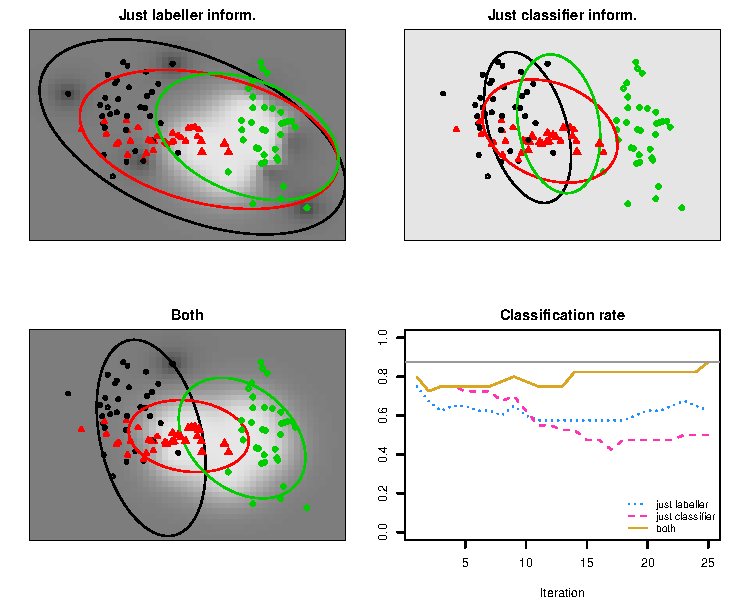
\includegraphics[width=6in]{figures/3_fields_and_tsplot.pdf}
\caption{Three results after 25 steps depending on which query
  strategy was used, and their classification rates on a test set as a
  function of steps. The horizontal line is for full training data
  with an oracle.}
\label{fig:four_square}
\end{figure}



\section{Application example}



\appendix
\bibliographystyle{plainnat}
\bibliography{references}

\end{document}






